% Graduation documentation
% Copyright 2016-2017, Sjors van Gelderen

% Document settings
% \documentclass[draft]{article}
\documentclass{article}
\author{Sjors van Gelderen}
\title{Exploring advanced programming concepts}
\date{\today{}}

% Packages
\usepackage[utf8]{inputenc}
\usepackage{amsmath}
\usepackage{listings}
\usepackage{float}
\usepackage[english]{babel}
\usepackage{csquotes}
\usepackage[backend=biber,style=numeric]{biblatex}
\addbibresource{bibliography.bib}
\usepackage{graphicx}
\graphicspath{{images/}}

% Content
\begin{document}

\maketitle{}


%%%%%%%%%%%%%%%%%%%%%%%%%%%%%%%%%%%%%%%%%%%%%%%%%%%%%%%%%%%%%%%%%%%%%%%%%%%%%%%%%%%%%%%%%%%%%%%%
\newpage


\tableofcontents{}


%%%%%%%%%%%%%%%%%%%%%%%%%%%%%%%%%%%%%%%%%%%%%%%%%%%%%%%%%%%%%%%%%%%%%%%%%%%%%%%%%%%%%%%%%%%%%%%%
\newpage


\section{Introduction}
In this document I describe the materials studied during my graduation phase. The aim of my research is to prepare
for professionally teaching students selective aspects of computer science. These aspects include:
\begin{enumerate}
\item{Data structures, algorithms and complexity analysis}
\item{Object-oriented design patterns}
\item{The {\em C\#} and {\em Python 3} programming languages}
\end{enumerate}

\paragraph{Relevance to video game development}
To write interesting software, the programmer must make clever use of the limited processing power available. Without data
structures and algorithms it is impossible to write meaningful and efficient programs. Well-designed data structures and
algorithms are what push the boundaries of the technology that drives video games.

\paragraph{Examples}
I have provided many example implementations in a variety of programming languages \cite{repo}.


%%%%%%%%%%%%%%%%%%%%%%%%%%%%%%%%%%%%%%%%%%%%%%%%%%%%%%%%%%%%%%%%%%%%%%%%%%%%%%%%%%%%%%%%%%%%%%%%


\subsection{Primary languages}
Here is a brief description of the main languages used.

\subsubsection{C\#}
This is Microsoft's highly popular \cite{popularity-index} {\em .NET} programming language. {\em C\#} can be considered a much
higher level variant of {\em C++}. With the rapidly growing {\em .NET} ecosystem and modern features such as {\em LINQ},
anonymous methods and {\em tasks}, {\em C\#} is certainly a powerful programming language.

\paragraph{Sources}
All {\em C\#} source code is provided in the subdirectory {\em csharp/}.

\subsubsection{Python 3}
Advantages of this language include its concise syntax and its portability. Because of {\em Python 3}'s high-level nature,
the programmer can focus exclusively on the actual logic of an algorithm rather than the low-level memory management involved.
This removes a significant source of potential distraction. For all its flexibility, it is error-prone. This means frequent
run-time debugging sessions are inevitable.

\paragraph{Sources}
All {\em Python 3} source code is provided in the subdirectory {\em python\_3/}.

\subsubsection{F\#}
Being a more recent addition to the {\em .NET} family of programming languages, {\em F\#} has not quite gained the popularity of
{\em C\#}. The {\em F\#} programming language enables the programmer to tackle problems using high-level concepts including
tail-recursion, higher order functions, partial application, currying, computation expressions (syntactic sugar for monads) and
more.

\paragraph{Sources}
All {\em F\#} source code is provided in the subdirectory {\em bonus/fsharp/}.


\subsection{Secondary languages}
These languages were only used sparingly, out of curiosity rather than necessity.

\subsubsection{C}
Virtually any programmer will at some point in their career encounter this venerable, fast and portable programming
language. Because this low-level language doesn't use a garbage collector, the programmer must exercise great caution
with the manual management of memory. Many security problems that affect us today are a direct consequence of the
programmer's failure to do so. This language is well-suited to studying the low-level implementation details of
algorithms and data structures.

\paragraph{Sources}
All {\em C} source code is provided in the subdirectory {\em bonus/c/}.

\subsubsection{Rust}
Developed by Mozilla, {\em Rust} aims to be a modern solution for safe, asynchronous programming.
With default immutable variables, as well as {\em borrowing} and {\em lifetimes}, the compiler makes it very
difficult indeed to write a program that contains run-time errors relating to incorrect memory access.

\paragraph{Sources}
All {\em Rust} source code is provided in the subdirectory {\em bonus/rust/}.

\subsubsection{Chicken Scheme}
The {\em LISP} family of programming languages has two major dialects; these being {\em Common LISP} and {\em Scheme}.
{\em Chicken Scheme} is a modern implementation of the {\em Scheme} dialect. It has a very minimalistic syntax,
revolving around the use of parentheses and prefix notation. {\em Chicken Scheme} is a high-level functional
programming language.

\paragraph{Sources}
All {\em Chicken Scheme} source code is provided in the subdirectory {\em bonus/chicken\_scheme/}.


%%%%%%%%%%%%%%%%%%%%%%%%%%%%%%%%%%%%%%%%%%%%%%%%%%%%%%%%%%%%%%%%%%%%%%%%%%%%%%%%%%%%%%%%%%%%%%%%
\newpage


\section{Analysis}

\subsection{Empirical analysis}
Empirical analysis is about inferring a program's expected performance based on measurements taken while running it. A typical
scenario involves the measurement of performance in terms of running time with a {\em stopwatch} program. By measuring the
performance with increasing {\em problem sizes} (generally the size of the input collection
\cite[p.25]{introduction-to-algorithms}) and plotting the results, an expected performance curve may be extrapolated.

\begin{figure}[H]
  \centering
  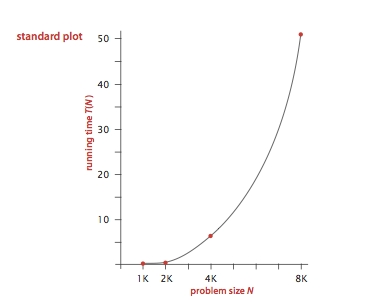
\includegraphics[width=8cm]{empirical_measurement}
  \caption{Empirical observations are used to plot a performance curve \cite[p.17]{empirical-analysis-princeton}}
\end{figure}

This technique may suffice if the target hardware is available for testing. If it is not, at least a simulation is necessary.
If neither of these is possible it will be difficult to get accurate measurements, because the hardware on which the experiments
are performed may differ greatly from the target hardware \cite[p.22]{empirical-analysis-princeton}.


\subsection{Complexity analysis}
Complexity analysis is different from empirical analysis in that it uses reasoning, rather than experiment, to determine
a program's expected performance. Using mathematical models, an algorithm can be analyzed and an expected performance class
may be inferred from the asymptotic growth of the function \cite[p.43-49]{introduction-to-algorithms}. There exist several
performance-related functions of interest:

\begin{samepage}
  \begin{figure}[H]
    \centering
    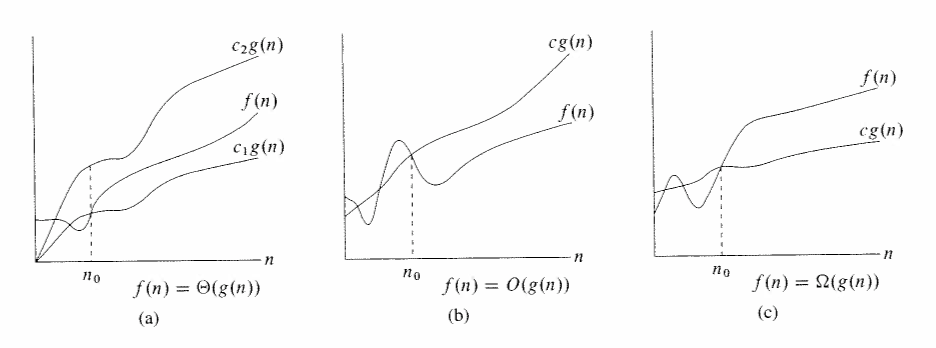
\includegraphics[width=10cm]{theta_o_omega}
    \caption{Functions used for analyzing different aspects of growth in a given complexity context
     \cite[p.45]{introduction-to-algorithms}}
  \end{figure}
  
  \paragraph{\(\boldsymbol \Omega\)}
  This symbol - pronounced {\em omega} - denotes a function that allows the programmer to determine the lower bound of a
  function's growth. The lower bound corresponds to the best case performance.
  
  \paragraph{\(\boldsymbol O\)}
  This symbol - pronounced {\em 'big oh'} - denotes a function that allows the programmer to determine the upper bound of a
  function's growth. The upper bound corresponds to the worst case performance.
  
  \paragraph{\(\boldsymbol \Theta\)}
  This symbol - pronounced {\em theta} - denotes a function that allows the programmer to determine both an upper and lower
  bound of a function's growth. The \(\Theta\) class corresponds to the average case performance.
\end{samepage}

\paragraph{}
All complexities provided in this document and related example implementations are worst case complexities. Although the other
complexity classes can help to provide a more complete estimation of the algorithm's actual performance, I have limited my
scope to the investigation of worst case (\(O\)) complexities for the following reasons
 \cite[p.27-28]{introduction-to-algorithms}:
\begin{enumerate}
\item{The worst case complexity provides the programmer with the guaranteed minimum performance}
\item{The worst case occurs frequently}
\item{The average case is usually close to the worst case}
\end{enumerate}

\subsection{Correctness}
In a mission-critical scenario, proving the correctness of algorithms is vital. This is done via the construction of a
mathematical proof. There exist many approaches to creating such a proof, but due to my limited mathematical background
this subject is unfortunately out of the scope of this document. Unless an algorithm is proven to be to correct, there
exists a chance that the algorithm will fail to provide the correct results.


%%%%%%%%%%%%%%%%%%%%%%%%%%%%%%%%%%%%%%%%%%%%%%%%%%%%%%%%%%%%%%%%%%%%%%%%%%%%%%%%%%%%%%%%%%%%%%%%
\newpage


\section{Data structures}
Any given implementation for an algorithm will expect a certain shape of data as its input. The shape of the data
can heavily affect the efficiency of a given operation. To control the shape of data, a programmer writes {\em data
structures}. In this section I describe various examples of common data structures.


\subsection{Array}
Among the most common data structures for collections is the array. All elements in the array are stored
{\em contiguously} in memory, and may be accessed in constant time(\(O(1)\)) through their respective indices.
Arrays have excellent {\em cache-alignment}, adding to their already excellent access time.

\begin{figure}[H]
  \centering
  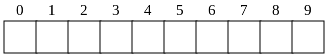
\includegraphics[width=6cm]{array}
  \caption{Array data structure with 0-based indices}
\end{figure}

The location of an element in an array at some given index {\em i} will be
\[base\_address\_of\_array + i * s\]
In which {\em s} is the size of a single element. This size depends on the type of data stored in the array.

\subsubsection{Size}
\paragraph{Fixed size}
By default, arrays are generally of {\em fixed size}. Since less elements might be stored in the array than its total
capacity allows for, space might be wasted on unused memory. The amount of elements that are actually being used is
called the {\em logical size} of the array.

\paragraph{Dynamic size}
When an array is of dynamic size, the programmer must carefully specify the amount by which the array will be resized.
If the programmer adds more elements than some given threshold will allow, the array must perform a resize operation.
Since the resize operation is costly (typically \(O(n)\)), frequent resizes ought to be avoided. In some implementations,
dynamic size arrays will also shrink when the logical size becomes less than a given threshold.

\subsubsection{Dimensionality}
Arrays may have more than one dimension. Such a construction is also be called a matrix. Elements in the multidimensional
array are be accessed with multiple indices describing the relevant coordinates.


%%%%%%%%%%%%%%%%%%%%%%%%%%%%%%%%%%%%%%%%%%%%%%%%%%%%%%%%%%%%%%%%%%%%%%%%%%%%%%%%%%%%%%%%%%%%%%%%


\subsection{Linked list}
The {\em linked list} is a linear, dynamic size data structure for storing collections of elements. Contrary to arrays,
elements are not guaranteed to be stored contiguously. This makes it possible to store elements in a fragmented fashion,
which is useful when the collection is larger than any available contiguous block of memory. Since elements in the linked
list are stored in a fragmented fashion, direct access through indices as done with the array becomes impossible.

\begin{figure}[H]
  \centering
  
\includegraphics[width=6cm]{linked_list}
  \caption{Singly-linked list data structure}
\end{figure}

The linked list consists of several segments, each of which has up to two references to other
elements in the sequence. The last element of the sequence will point to an empty segment,
which may be called a {\em null link}. Traversing the linked list is a linear time (\(O(n)\)) operation.

\paragraph{Singly-linked and doubly-linked}
The {\em singly-linked} list consists of segments that contain a value and a reference to the next
segment in the sequence. The {\em doubly-linked} list is the same as the singly-linked list,
except each segment also has a reference to the previous segment in the sequence.
Whether the list is singly-linked or doubly-linked affects the traversal process,
since where singly-linked lists only allow forward traversal, doubly-linked lists also allow backward traversal.

\paragraph{Insert}
Elements are inserted at the root of the list. Since no traversal is required to locate the root,
the insertion operation is of constant time \(O(1)\). The inserted element becomes the new root,
and is given a reference to the next segment. This next segment is the old root segment.

When inserting at the end - rather than the beginning - of a list, the list must be traversed until a given segment
references a null link as the next element in the sequence. The reference to the empty segment may be replaced with
a reference the element to be inserted. Due to the traversal, the worst case complexity of such an insertion is of
linear time \(O(n)\). If the list is {\em doubly-linked}, the new element's {\em previous} variable should reference
the last element of the current list.

\paragraph{Delete}
Locating the element to be deleted will in the worst case require a complete traversal of the list,
which is a linear time (\(O(n)\) operation. If the current segment's {\em next} variable references
the element to be deleted, it must be changed to point to the segment in the sequence that succeeds
the element to be deleted (which may be {\em null}). If the root element is deleted, the next segment
in the list becomes the root.


%%%%%%%%%%%%%%%%%%%%%%%%%%%%%%%%%%%%%%%%%%%%%%%%%%%%%%%%%%%%%%%%%%%%%%%%%%%%%%%%%%%%%%%%%%%%%%%%


\subsection{Stack}
The {\em stack} is a {\em LIFO} (Last In, First Out) data structure. Data is always inserted on and removed
from the top of the stack. Only the top element of the stack may be inspected at any time. Regardless of which
structure is used to store the stack contents, the interface must always offer the following operations:
{\em push}, {\em pop} and {\em peek}.

\begin{figure}[H]
  \centering
  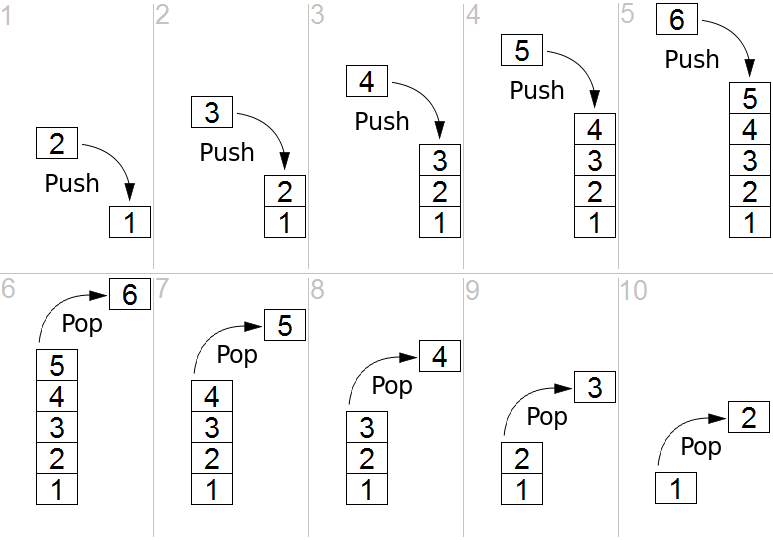
\includegraphics[width=10cm]{stack}
  \caption{Stack data structure and the workings of its operations}
\end{figure}

\paragraph{Push}
The {\em push operation} puts a new element on top of the stack. This is a constant time (\(O(1)\)) operation.
If the stack has a size limit, this operation throws a {\em stack overflow} exception when the stack's capacity
is exceeded.

\paragraph{Pop}
The pop operation removes the top element from the stack. This is a constant time (\(O(1)\)) operation.
If the stack has no elements, this operation will throw a {\em stack underflow} or {\em invalid operation}
exception, as there are no elements to remove.

\paragraph{Peek}
The peek operation gives the programmer access to the current top element of the stack.
This is a constant time (\(O(1)\)) operation. If the stack is empty, this operation will throw an
{\em invalid operation} exception, as there are no elements on the stack to reveal.

\begin{samepage}
  \paragraph{Sources}
  Stack implementations are provided at the following locations:
  \begin{itemize}
  \item{{\em csharp/data\_structures/stack/}}
  \item{{\em python\_3/data\_structures/}}
  \item{{\em bonus/c/data\_structures/}}
  \item{{\em bonus/fsharp/data\_structures/}}
  \end{itemize}
\end{samepage}


%%%%%%%%%%%%%%%%%%%%%%%%%%%%%%%%%%%%%%%%%%%%%%%%%%%%%%%%%%%%%%%%%%%%%%%%%%%%%%%%%%%%%%%%%%%%%%%%


\subsection{Queue}
Contrary to the stack, the queue is a {\em FIFO} (First In, First Out) data structure.
Elements are inserted at the back of the queue, and removed from the front of the queue.

\begin{figure}[H]
  \centering
  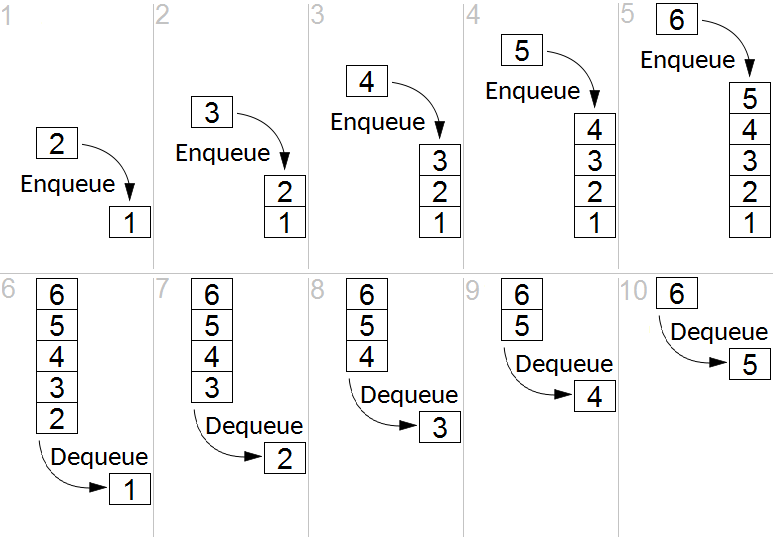
\includegraphics[width=10cm]{queue}
  \caption{Queue data structure and the workings of its operations}
\end{figure}

\paragraph{Enqueue}
The {\em enqueue} operation adds a new element at the front of the queue.
This is a constant time (\(O(1)\)) operation.

\paragraph{Dequeue}
The {\em dequeue} operation removes the element at the back of the queue.
This is a constant time (\(O(1)\)) operation for arrays, and a linear time (\(O(n)\)) for linked-lists.

\paragraph{IsEmpty}
The {\em is\_empty} operation returns whether the queue is empty or not.
This is a constant time (\(O(1)\)) operation. It can be used to prevent queue underflow.

\paragraph{Rear and front}
The {\em rear} and {\em front} operations provide access to the front and rear elements of the queue.
These operations are optional and as such are not provided in all implementations. Both operations are
constant time (\(O(1)\)) operations for arrays. The rear operation is linear time (\(O(n)\)) and the
front operation is constant time (\(O(1)\)) for linked-lists.

\begin{samepage}
  \paragraph{Sources}
  Queue implementations are provided at the following locations:
  \begin{itemize}
  \item{{\em csharp/data\_structures/queue/}}
  \item{{\em python\_3/data\_structures/}}
  \item{{\em bonus/c/data\_structures/}}
  \item{{\em bonus/fsharp/data\_structures/}}
  \end{itemize}
\end{samepage}


%%%%%%%%%%%%%%%%%%%%%%%%%%%%%%%%%%%%%%%%%%%%%%%%%%%%%%%%%%%%%%%%%%%%%%%%%%%%%%%%%%%%%%%%%%%%%%%%


\subsection{Hashmap}
This data structure - also known as a {\em dictionary} or {\em hash table} - is used to store a list of
key-value pairs. This kind of structure is also called an {\em associative array}. The data structure
consists of a list or array of {\em buckets} or {\em slots} containing one or more elements. The amount
of elements that may be stored in a given bucket depends on the implementation of said bucket.
The underlying data structure may, for example, be a fixed-size array or a linked-list.

\begin{figure}[H]
    \centering
    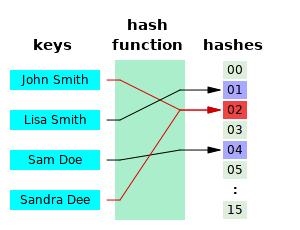
\includegraphics[width=6cm]{hash_map}
    \caption{Hashmap data structure}
\end{figure}

\begin{samepage}
  Of primary interest is the way the indices of the relevant bucket are determined. Unlike standard arrays,
  indices need not be integers. Indices may instead be derived from any kind of data type. This is done using
  a {\em hash function} (hence, the name of the data structure). The hash function derives an integer from the
  provided data. The modulo operator then restricts the provided integer to a range that fits in the array or list.
  
  \begin{equation}
    hash\_value = hash\_function(data)
  \end{equation}
  
  \begin{equation}
    hash\_map\_index = hash\_value \ \% \ hash\_map\_size
  \end{equation}
\end{samepage}

\begin{samepage}
  To determine whether the number of buckets is appropriate for the amount of elements to be inserted,
  the load factor may be calculated. The load factor is calculated as follows:
  
  \begin{equation}
    \frac{number\_of\_entries}{number\_of\_buckets}
  \end{equation}

  \paragraph{}
  A large load factor is indicative of an inappropriate amount of buckets.
  If the load factor is too small, however, it is possible a lot of buckets are unnecessarily taking up space.
  Some implementations of hash maps will resize when the load factor reaches a certain threshold.
  This is a costly operation, seeing as all elements will have to be redistributed according to the new size.
\end{samepage}

\begin{figure}[H]
  \centering
  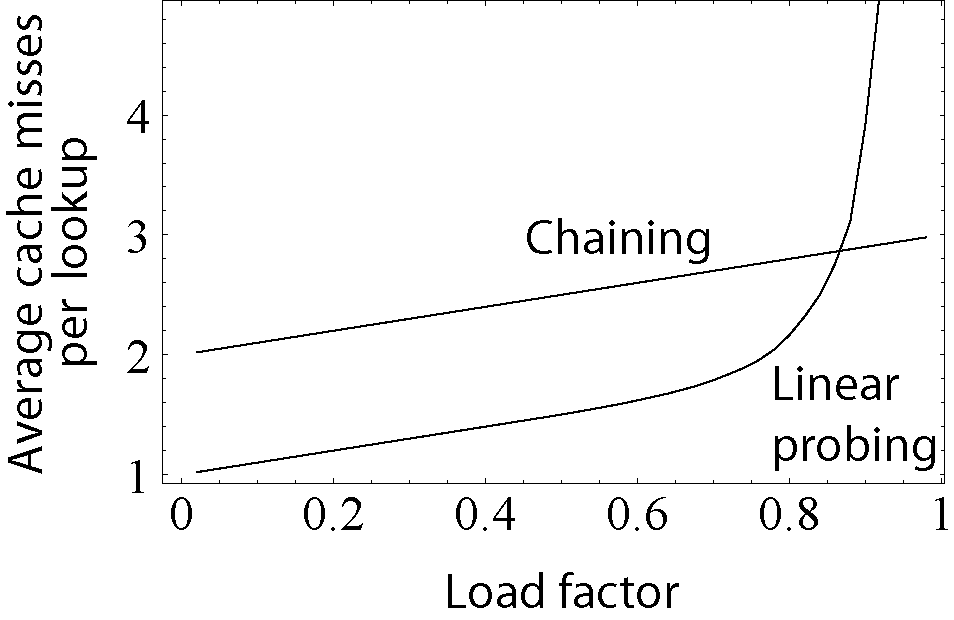
\includegraphics[width=6cm]{load_factor}
  \caption{Diagram of several aspects of the hashmap}
\end{figure}

It is possible that two different pieces of data generate the same hash map index.
Such a situation is called a {\em collision}. If there are many collisions, the distribution of the values
will be poor. As a consequence, the data structure will be inefficient.
If all keys are known before the data is inserted into the hash map, it is possible to generate a perfect
hashing function. This means each piece of data provided will result in a unique hash map index.

\paragraph{Collision resolution}
There exist several solutions to the collision problem, three of which are described in the next sections.

\subparagraph{Linear and quadratic probing}
When performing {\em linear probing}, a collision causes the hash map index to be increased successively by one,
until an empty bucket is found. Similarly, {\em quadratic probing} successively increases the hash map index using
values from a quadratic polynomial to find an appropriate bucket for the colliding element. Usually both of these
probing methods will wrap around if the resulting hash map index is outside of the range of the bucket array.
These methods may cause elements to occupy buckets that would otherwise be populated by other pieces of data.
In addition, these probing methods may cause infinite loops when an acceptable bucket is never found.

\subparagraph{Dynamic size buckets}
Another solution to the collision problem is to allow multiple values per bucket. Such a solution could be
implemented by making each bucket into a dynamic size array or linked list. If hash function or load-factor is bad,
this implementation may result in similar efficiency to simply using a single dynamic size array or linked list.


%%%%%%%%%%%%%%%%%%%%%%%%%%%%%%%%%%%%%%%%%%%%%%%%%%%%%%%%%%%%%%%%%%%%%%%%%%%%%%%%%%%%%%%%%%%%%%%%


\subsection{Tree}
Trees are hierarchical data structures consisting of {\em linked nodes}. Unless the tree is empty, there will be a
top node called the {\em root node}. From this node spring all the {\em subtrees}. Any node other than the root node
of the tree is called a {\em child node}. The predecessor of a child node is called its {\em parent}. The root node
is the only node that does not have a parent. Nodes that don't have any children are called {\em leaves}, expanding
on the analogy of the tree. Any node that has at least one child is an {\em internal node}. A tree is said to be
{\em balanced} if the nodes are distributed evenly among the subtrees in the tree. A tree might be so poorly
balanced that the nodes are organized much like a {\em linked list}. In this case, it's possible that the tree was
not a suitable data structure for the relevant problem. The {\em depth} of a node is the amount of {\em edges} that
must be traversed from the root to reach it. A collection of edges to traverse is called a {\em path}, the length of
which is the amount of edges. All nodes of the same depth are said to be on the same {\em level}.
In this section are described a number of data structures that may be called trees.


\begin{samepage}
\subsubsection{Binary tree}
The binary tree - also called {\em bifurcating arborescence} - consists of nodes containing at most one parent,
and at most two children. There is no particular property governing where new elements are inserted. This is because
the binary tree does not inherently imply any particular sorting order. A binary tree is said to be {\em full} if
all of its leaves are on the same level, and each internal node has two children. This is different from the notion
of completeness, as a {\em complete} binary tree is a tree where each level other than possibly the last is fully
populated, and all nodes are as far to the left as possible.

\begin{figure}[H]
  \centering
  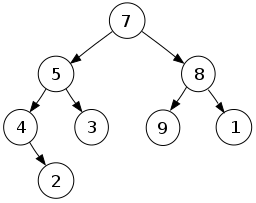
\includegraphics[width=6cm]{binary_tree}
  \caption{Binary tree data structure}
\end{figure}

\paragraph{Sources}
A binary tree implementation is provided at the following location:
\begin{itemize}
  
\item{{\em bonus/fsharp/data\_structures/}}
\end{itemize}
\end{samepage}


\subsubsection{Binary heap}
This complete binary tree maintains the {\em heap property}, which is said to be {\em max} or {\em min}.
A heap that satisfies the {\em max heap property} is called a {\em max heap}.
Accordingly, a heap that satisfies the {\em min heap property} is called a {\em min heap}.
The property determines the order in which the elements are stored inside the heap.

\begin{figure}[H]
  \centering
  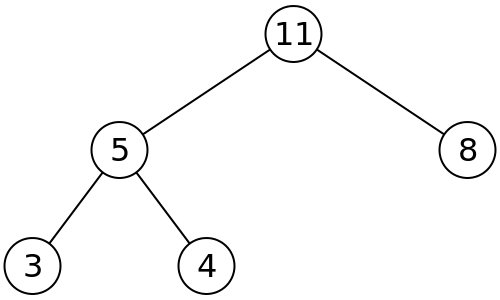
\includegraphics[width=6cm]{binary_heap}
  \caption{Diagram of a binary max heap}
\end{figure}

In a max heap each key must be greater than every key stored inside its children.
Conversely, in a min heap each key must be less than every key stored inside its children.

\paragraph{Insert}
The {\em insert} operation adds a new key at the end of the heap. If the heap property is violated,
it may be restored by letting the key 'swim' to the correct position. When 'swimming', the key
is compared to its parent. If the a violation of the heap property is found, the key and its parent
are swapped. This process is repeated until the heap property is no longer violated. Note that the
heap property is also restored if this key becomes the new root of the heap. This is an \(O(log n)\)
operation.

\paragraph{Extract and heapify}
The {\em extract} operation removes the root node from the binary heap. It does this by replacing
the root key with the last key in the heap. After this step, the {\em heapify} operation is used to
restore the heap property if it is be violated by the new root. In such case, the root is compared
to its children. Depending on the relevant property, the root is swapped with either its smaller child in a
min-heap, or its larger child in a max heap. The process is then repeated from the old root's new location,
which is the index of the child it was swapped with. Eventually, the heap property must be restored.
This is a \(O(log n)\) operation.

\paragraph{Sources}
Heap implementations are provided at the following locations:
\begin{itemize}
\item{{\em csharp/data\_structures/heap/}}
\item{{\em python\_3/data\_structures/}}
\item{{\em bonus/fsharp/data\_structures/} (At the time of writing incomplete)}
\end{itemize}


\subsubsection{Binary search tree}
Similar to the binary heap, the binary search tree must satisfy an ordering principle: the binary search tree
property. This property allows for more efficient searching algorithms, as the partitioning of the tree is known.
The binary search tree property states that all keys in the children of the current node must be less than the key
of the current node, and all keys in the right children of the current node must be greater than the key of the
current node. In a standard implementation, duplicate values are generally not allowed.

\begin{figure}[H]
    \centering
    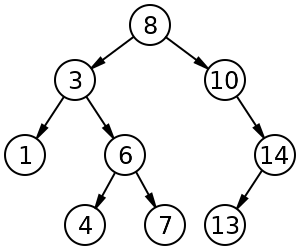
\includegraphics[width=6cm]{binary_search_tree}
    \caption{Binary search tree}
  \end{figure}

\begin{samepage}
  \paragraph{Traversals}
  Visiting elements in a tree is called {\em traversing} the tree. The most common traversals are the following:

  \subparagraph{Pre-order traversal}
  Visit the root, visit the left subtree, visit the right subtree.

  \begin{figure}[H]
    \centering
    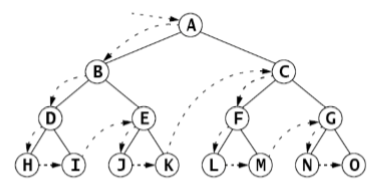
\includegraphics[width=4cm]{pre_order_traversal}
    \caption{Pre-order traversal diagram}
  \end{figure}

  \subparagraph{In-order traversal}
  Visit the left subtree, visit the root, visit the right subtree.

  \begin{figure}[H]
    \centering
    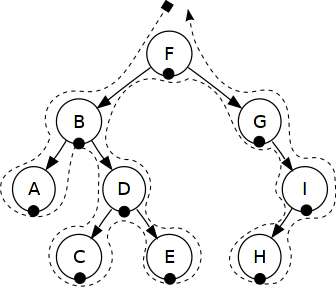
\includegraphics[width=4cm]{in_order_traversal}
    \caption{In-order traversal diagram}
  \end{figure}

  \subparagraph{Post-order traversal}
  Visit the left subtree, visit the right subtree, visit the root.

  \begin{figure}[H]
    \centering
    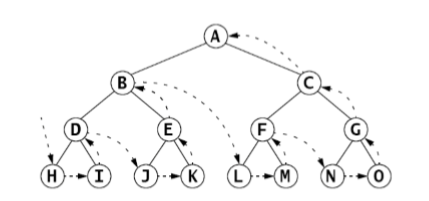
\includegraphics[width=4cm]{post_order_traversal}
    \caption{Post-order traversal diagram}
  \end{figure}
\end{samepage}

\paragraph{Insert}
The {\em insert} operation is used to insert new keys into the tree. This is a linear time (\(O(n)\)) operation.
Since the binary search tree property must be maintained, the insert operation has to intelligently locate the
correct position for the new element. The insert operation always starts from the root of the tree,
which may be empty. If the current node is not empty, the algorithm will continue on the left subtree if
the value to be inserted is less than the value in the current key. Otherwise, it will continue on the right
subtree. This process is repeated until an empty node is found. When it is found, the new element will populate
the empty node.

\paragraph{Delete}
The {\em delete} operation is used to delete existing keys from the tree. This is a linear time (\(O(n)\))
operation. First, the element to be deleted must be located. Once the target key is found, the algorithm must
establish how to proceed with the deletion. If the node to be deleted does not have any children, the delete
operation is trivial, as the current node can simply be erased. If the node has a single child, that child will
take the place of the node to be deleted. A more complex situation occurs if the node has two children, as the
binary search tree property must be maintained. To do this, the algorithm must either locate the
{\em in-order successor} or {\em in-order predecessor} of the target node. The located node's key then replaces
the deletion target node's key. After this, the delete operation continues on the located node until one of the
trivial cases occurs.

\paragraph{Search}
The {\em search} operation is a linear time (\(O(n)\)) operation that finds a target node based on its key.
Since the binary search tree property holds, the search operation may from any key easily determine whether to
branch the search operation to the left or right of said node. If an empty node is encountered, the key is
not in the tree.

\begin{samepage}
  \paragraph{Sources}
  Binary search tree implementations are provided at the following locations:
  \begin{itemize}
  \item{{\em csharp/data\_structures/binary\_search\_tree/}}
  \item{{\em python\_3/data\_structures/}}
  \item{{\em bonus/c/data\_structures/}}
  \item{{\em bonus/fsharp/data\_structures/}}
  \end{itemize}
\end{samepage}


\subsubsection{K-dimensional tree}
The {\em K-dimensional} tree expands upon the philosophy of the binary search tree, in that it
must maintain a sorting order property. When using this tree in less than 4 dimensions,
a simple geometric interpretation of its structure is possible. Beyond this, the analogy becomes
more difficult to grasp as it involves the splitting of hyperplanes.

\paragraph{Insert}
The {\em insert} operation of a K-dimensional tree is of linear time (\(O(n)\)).
Let's examine the construction of a {\em 2-dimensional} tree from the array \(A = [(3, 2), (6, 5), (7, 1)]\).
The root key of the tree will be the first element in the array, in this case \((3, 2)\).
We will record this key as a {\em vertical} split of the plane, like so:

\begin{figure}[H]
  \centering
  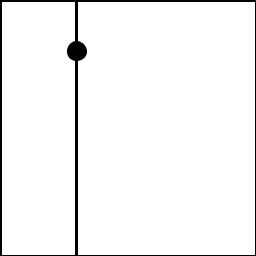
\includegraphics[width=4cm]{2d_tree_0}
  \caption{Node \((3, 2)\) is splitting the plane vertically}
\end{figure}

Since the next key in the collection - \((6, 5)\) - has a larger \(X\) coordinate than the root key(\(6 > 3\)),
it will be stored to the left of the root key. Notice that this operation has added a new level to our tree.
In a 2-dimensional tree each level of the tree will be recorded as being either {\em vertical} or {\em horizontal}.
For this example, let's assume that even levels are vertical, whereas odd levels are horizontal.

\begin{figure}[H]
  \centering
  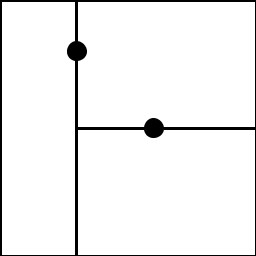
\includegraphics[width=4cm]{2d_tree_1}
  \caption{Node \((6, 5)\) is splitting the subsection of the plane horizontally}
\end{figure}

The next key in our collection - \((7, 1)\) - has a larger \(X\) coordinate than our root key(\(7 > 3\)),
and so the key must be stored in the right subtree. The right subtree is not empty,
therefore we must compare the right child of the root key to the key we're inserting.
Since the right child of the root key is on an odd level in our tree, it corresponds to a {\em horizontal} split.
The consequence of this difference is that we must now compare the \(Y\) coordinates - rather than the \(X\)
coordinates - of our keys. Since the \(Y\) coordinate of our insertion key is less than that of the right child
of the root key, we must store our new element to the left of the right child of the root key.

\begin{figure}[H]
  \centering
  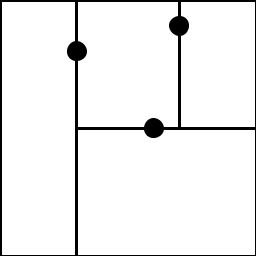
\includegraphics[width=4cm]{2d_tree_2}
  \caption{Node \((7, 1)\) is making yet another vertical split}
\end{figure}

\paragraph{Search}
The {\em search} operation for a key on a k-dimensional tree is of linear time (\(O(n)\)).
When searching for a key, the orientation of each level must be taken into account.
Similar to the insertion operation, the \(X\) or \(Y\) coordinates will be compared to determine
whether the left or right subtree is to be used for the rest of the search operation.
If they key is encountered, the search is succesful. If an empty tree is encountered instead,
the search was not succesful as the key is not in the tree.

\paragraph{Range query}
The {\em range query} operation is of \(O(\sqrt{n} + k)\) time complexity, where \(k\) denotes the number of
reported points. In the 2-dimensional tree, this operation queries a rectangular section of the plane and
returns the points contained within that section.

\begin{figure}[H]
  \centering
  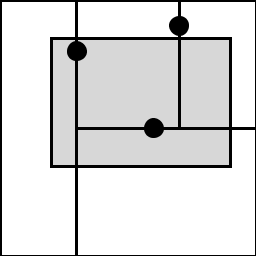
\includegraphics[width=4cm]{2d_tree_3}
  \caption{A range query is performed on the rectangular area \((2, 1.5, 9, 6.5)\)}
\end{figure}

As with the operation that searches for a single key, the range query must take notice of the orientation
associated with each level. Rather than always continuing the query on a single child tree,
the range query may continue on both children if the section covers space on both sides of the current key's split.

\begin{samepage}
  \paragraph{Sources}
  A K-dimensional search tree implementation is provided at the following location:
  \begin{itemize}
  \item{{\em csharp/data\_structures/kd\_tree/}}
  \end{itemize}
\end{samepage}


%%%%%%%%%%%%%%%%%%%%%%%%%%%%%%%%%%%%%%%%%%%%%%%%%%%%%%%%%%%%%%%%%%%%%%%%%%%%%%%%%%%%%%%%%%%%%%%%


\subsection{Graph}
The {\em graph} may be used to represent a relational network of nodes called {\em vertices}.
Vertices are connected via {\em edges}. Vertices that are connected to each other via a single edge are called
{\em adjacent} or {\em neighbors}. A collection of edges connecting two vertices is a {\em path}. The graph does
not imply any particular root, nor does it restrict the number of edges connecting any vertex to other vertices.

\begin{figure}[H]
  \centering
  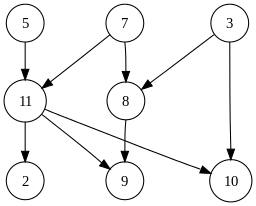
\includegraphics[width=6cm]{graph_0}
  \caption{A directed acyclic graph without weights}
\end{figure}

\subsubsection{Weighted}
A graph is {\em weighted} if each of its edges has a 'cost' associated with traversing it. Such graphs may,
for instance, be used to map distances between locations on a map.

\subsubsection{Directed}
A graph is {\em directed} if each of its edges has an associated direction. This direction implies a restriction
on the traversal, as only the direction given for each edge is allowed to be travelled. A directed graph is also
called a {\em digraph}.

\subsubsection{Dense versus sparse}
Graphs are called {\em dense} if there are many edges connecting many vertices. Conversely, a graph may be called
{\em sparse} if there are comparatively few edges connecting the vertices.

\begin{figure}[H]
  \centering
  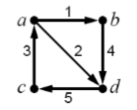
\includegraphics[width=4cm]{weighted_directed_graph}
  \caption{The weighted digraph used in the following examples. In some examples, the direction is ignored}
\end{figure}

\subsubsection{Adjacency list}
Graphs may be structured as an {\em adjacency list}. This is a list of vertices, each of which is associated with
all of its neighbors.

\begin{figure}[H]
  \centering
  \begin{tabular}{|c|c c c|}
    \hline
    A  & B & C & D  \\ [0.5ex]
    \hline
    B  & A & D & \  \\
    \hline
    C  & D & A & \  \\
    \hline
    D  & C & B & A  \\
    \hline
  \end{tabular}
  \quad
  \begin{tabular}{|c|c c|}
    \hline
    A  & B & D  \\ [0.5ex]
    \hline
    B  & D & \  \\
    \hline
    C  & A & \  \\
    \hline
    D  & C & \  \\
    \hline
  \end{tabular}
  \caption{Examples of adjacency lists. The right list is for a digraph}
\end{figure}

The adjacency list is the preferred representation when the graph is sparse. In a digraph, only edges that {\em emanate from}
(start at) the vertex are recorded for that vertex.

\subsubsection{Adjacency matrix}
The {\em adjacency matrix} is a multi-dimensional array. The axes both contain each vertex in the graph. If two vertices are
adjacent, it is recorded in the matrix. The recorded value may be a boolean type, in which case the value is \(true\) if the
vertices are adjacent. If the graph is weighted, the value may contain the weight of the connecting edge instead of the boolean
value. In this case, the weight for non-adjacent vertices could be recorded as being infinite.

\begin{figure}[H]
  \centering
  \begin{tabular}{|c|c|c|c|c|}
    \hline
    \  & A & B & C & D \\ [0.5ex] 
    \hline
    A  & F & T & T & T \\ 
    \hline
    B  & T & F & F & T \\
    \hline
    C  & T & F & F & T \\
    \hline
    D  & T & T & T & F \\
    \hline
  \end{tabular}
  \quad
  \begin{tabular}{|c|c|c|c|c|}
    \hline
    \  & A          & B          & C          & D          \\ [0.5ex] 
    \hline
    A  & \(infty\)  & 1          & \(\infty\) & 2          \\ 
    \hline
    B  & \(\infty\) & \(\infty\) & \(\infty\) & 4          \\
    \hline
    C  & 3          & \(\infty\) & \(\infty\) & \(\infty\) \\
    \hline
    D  & \(\infty\) & \(\infty\) & 5          & \(\infty\) \\
    \hline
  \end{tabular}
  \caption{Examples of adjacency matrices. The right matrix is for a weighted graph}
\end{figure}

The adjacency matrix is the preferred representation when the graph is dense.

\subsubsection{Incidence matrix}
The {\em incidence matrix} shows the relationship between vertices (represented in the rows) and edges (represented in the
columns) in a graph. If the vertices are {\em incident upon} (connected to) the edge, a boolean value or weight is be recorded
in the matrix. In a digraph, edges that emanate from the row vertex are given the value 1. Edges that {\em terminate at} (end
at) the row vertex are instead given the value -1.

\begin{figure}[H]
  \centering
  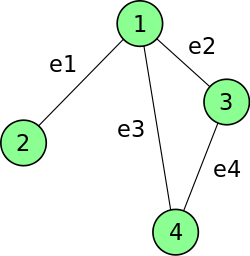
\includegraphics[width=4cm]{incidence_graph}
  \caption{The graph described by the incidence matrix}
\end{figure}

\begin{figure}[H]
  \centering
  \begin{tabular}{|c|c|c|c|c|c|}
    \hline
    \  & e1 & e2 & e3 & e4 \\ [0.5ex]
    \hline
    A  & T  & T  & T  & F  \\ 
    \hline
    B  & T  & F  & F  & F  \\
    \hline
    C  & F  & T  & F  & T  \\
    \hline
    D  & F  & F  & T  & T  \\
    \hline
  \end{tabular}
  \caption{Example of an incidence matrix}
\end{figure}


\subsubsection{Traversal}
Here are listed two ways to visit each vertex in a graph,
both of which are of linear time (\(O(n)\)) complexity.

\paragraph{Breadth-first search}
The {\em breadth-first search} uses the {\em queue} data structure. The general procedure is as follows:
\begin{enumerate}
\item{Enqueue the root vertex}
\item{Dequeue a vertex. If this is the target, stop the search. Otherwise, enqueue all unvisited direct children}
\item{If the queue is empty, the traversal is complete and the search was unsuccesful. Otherwise repeat step 2}
\end{enumerate}

\begin{figure}[H]
  \centering
  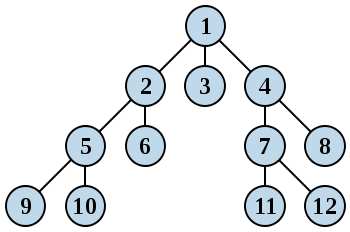
\includegraphics[width=6cm]{breadth_first_search}
  \caption{Order of visited vertices in a graph using breadth-first search \cite{bfs}}
\end{figure}

\paragraph{Depth-first search}
The {\em depth-first traversal} uses the {\em stack} data structure. The general procedure is as follows:
\begin{enumerate}
\item{Start at the root vertex}
\item{If the current vertex is the target, stop the search. Otherwise, continue at step 3}
\item{Push the first unvisited neighboring vertex onto the stack}
\item{Repeat step 3 until no more unvisited neighbors exist, then pop from the stack. Repeat from step 2}
\end{enumerate}

\begin{figure}[H]
  \centering
  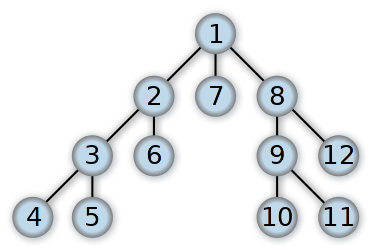
\includegraphics[width=6cm]{depth_first_search}
  \caption{Order of visited vertices in a graph using depth-first search \cite{dfs}}
\end{figure}


%%%%%%%%%%%%%%%%%%%%%%%%%%%%%%%%%%%%%%%%%%%%%%%%%%%%%%%%%%%%%%%%%%%%%%%%%%%%%%%%%%%%%%%%%%%%%%%%
\newpage


\section{Algorithms}
Executable instructions for transforming some input to some output are called {\em algorithms}
 \cite[p.5]{introduction-to-algorithms}. Many algorithms may exist for solving a given problem, but some will be better suited
to the task than others.

\paragraph{Complexity}
When measuring {\em complexity}, a programmer measures how a given factor scales according to the problem {\em problem size}.
An example of a problem size is the size of the input collection for a sorting algorithm. The most common categories to measure
are {\em time complexity}, which has to do with the {\em running time} of an algorithm, and {\em space complexity}, which
reveals how much memory the algorithm will occupy according to the problem size.

\paragraph{Divide-and-conquer}
Algorithms that cut the problem into several subproblems in order to speed up the process are called {\em divide-and-conquer}
algorithms \cite[p.30-38]{introduction-to-algorithms}. Examples of divide-and-conquer algorithms include merge sort and binary
search.

\paragraph{Stability}
The concept of {\em stability} in a sorting algorithm has to do with maintaining the original order of duplicate entries in the
input collection. Imagine a hand of cards containing both an ace of spades and an ace of clubs. These cards share their rank,
but not their suit. The sorting algorithm might sort according to rank only. In a stable sort, the cards must appear in the same
order with respect to each other after the sorting algorithm is complete.

\paragraph{Greedy algorithms}
Some algorithms will quickly find a result, but they are so {\em greedy} that the result is sub-optimal. If the result need
not be completely accurate, greedy algorithms sometimes offer a fast alternative to their more meticulous counterparts.


\subsection{Searching}
\subsubsection{Linear search}
The {\em linear search} traverses a collection in linear fashion until either the requested element is found,
or the end of the collection was reached. This is a linear time (\(O(n)\)) operation.
Linear search is simple to implement and is well-suited to small unsorted collections.

\paragraph{Setup}
This algorithm expects as input a collection of keys and a target key to find in the collection. An index is used to keep track
of which key is to be scanned next.

\paragraph{Process}
\begin{enumerate}
\item{If the index is outside of the bounds of the collection, the search is complete but the target key was not found.
  Otherwise, continue from step 2}
\item{If the key at the current index in the collection is the target key, the search is complete and the target key was found.
  Otherwise, continue from step 3}
\item{Increment the index and continue from step 1}
\end{enumerate}

\begin{samepage}
  \paragraph{Sources}
  Linear search implementations are provided at the following locations:
  \begin{itemize}
  \item{{\em csharp/algorithms/searching/}}
  \item{{\em python\_3/algorithms/}}
  \item{{\em bonus/c/algorithms/}}
  \item{{\em bonus/fsharp/algorithms/}}
  \item{{\em bonus/rust/searching/}}
  \item{{\em bonus/chicken\_scheme/algorithms/}}
  \end{itemize}
\end{samepage}

\subsubsection{Binary search}
If the collection is known to be sorted, the {\em binary search} algorithm may yield a significant performance
gain compared to regular insertion sort. This is because the algorithm can use a pivot to intelligently search
the collection. This is a logarithmic time (\(O(log n)\)) operation.

\paragraph{Setup}
This algorithm expects as input a sorted collection of keys, a starting position for the pivot and the target key to find in
the collection.

\paragraph{Process}
\begin{enumerate}
\item{If the key at the pivot is the target key, the search is complete. Otherwise, continue from step 2}
\item{If the key is less than the key at the pivot, the pivot becomes the middle of the collection's segment to the left of the
    pivot. Otherwise, the pivot will become the middle of the collection's segment to the right of the pivot}
\item{If the pivot is the same as it was in the last iteration, the search is complete, but the key was not found. Otherwise,
    continue from step 1}
\end{enumerate}

\begin{samepage}
  \paragraph{Sources}
  \begin{itemize}
  \item{{\em csharp/algorithms/searching/}}
  \item{{\em python\_3/algorithms/}}
  \item{{\em bonus/rust/algorithms/searching/}}
  \end{itemize}
\end{samepage}


\subsection{Sorting}
Here are described various sorting algorithms of which I have provided implementations in various programming
languages.

\subsubsection{Insertion sort}
Perhaps the most basic sorting algorithm is {\em insertion sort}. Insertion sort must in the worst case compare
each element to every other element in the collection. It is therefore of quadratic time (\(O(n^2)\)) complexity.
The process is frequently compared to the steps involved in sorting a hand of playing cards.

\paragraph{Setup}
This algorithm expects as input a linear collection of sortable keys.

\paragraph{Process}
For each element in the collection:
\begin{enumerate}
\item{If the key has a left-side neighbor, compare it to that neighbor}
\item{If the key is smaller than its neighbor, swap them}
\item{Repeat from step 1 until either no more neighbor exists, or the key is larger than its neighbor}
\end{enumerate}

\begin{samepage}
  \paragraph{Sources}
  \begin{itemize}
  \item{{\em csharp/algorithms/searching/}}
  \item{{\em python\_3/algorithms/}}
  \item{{\em bonus/fsharp/algorithms/}}
  \item{{\em bonus/rust/algorithms/searching/}}
  \end{itemize}
\end{samepage}

\subsubsection{Shell sort}
The {\em shell sort} algorithm utilizes insertion sort in a divide-and-conquer strategy.
Shell sort is a \(O(n log^2 n)\) time complexity algorithm.

\paragraph{Setup}
The algorithm expects as inputs a collection of sortable keys and a slice size. The collection will be cut up into
slices according to the provided size. The results are stored into a buffer list or array.

\paragraph{Process}
\begin{enumerate}
\item{For each slice:}
  \begin{enumerate}
  \item{Run insertion sort on the slice}
  \item{Once complete, concatenate the sorted slice to the buffer}
  \end{enumerate}
\item{Run insertion sort on the buffer}
\end{enumerate}

\begin{samepage}
  \paragraph{Sources}
  \begin{itemize}
  \item{{\em csharp/algorithms/shell\_sort/}}
  \item{{\em python\_3/algorithms/}}
  \end{itemize}
\end{samepage}


\subsubsection{Bubble sort}
The {\em bubble sort} algorithm lets elements in an unsorted collection 'bubble' up to the correctly sorted position
in the resulting collection. Bubble sort is of quadratic time (\(O(n^2)\)) complexity.

\paragraph{Setup}
The algorithm expects as input an unsorted collection. It keeps track of an index indicating how many keys are
already sorted.

\paragraph{Process}
Until the index is equal to the size of the collection:
\begin{enumerate}
\item{Take a slice from the index to the end of the collection and increment the index}
\item{Take the rightmost key of the slice}
\item{If the key does not have a left-side neighbor, continue from step 1}
\item{If the left-side neighbor is smaller than the key, swap the keys}
\item{Continue from step 3}
\end{enumerate}

\begin{samepage}
  \paragraph{Sources}
  \begin{itemize}
  \item{{\em csharp/algorithms/bubble\_sort/}}
  \item{{\em python\_3/algorithms/}}
  \end{itemize}
\end{samepage}


\subsubsection{Comb sort}
The {\em comb sort} algorithm addresses a problem bubble sort faces when dealing with small values near the end of
the unsorted input collection. Comb sort is a quadratic time (\(O(n^2)\)) complexity algorithm.

\paragraph{Setup}
The algorithm expects as input an unsorted collection of keys and a gap shrink factor. The first gap size is the
length of the input collection multiplied by the shrink factor.

\paragraph{Process}
\begin{enumerate}
\item{Multiply the gap size by the shrink factor}
\item{If the gap size is smaller than or equal to 1 the algorithm is finished}
\item{Set an index to 0}
\item{If the index plus the gap size is larger than or equal to the length of the collection, continue from step 1}
\item{If the key at the current index in the collection is larger than the key at the index plus the gap size,
  swap those keys}
\item{Increment the index and continue from step 4}
\end{enumerate}

\begin{samepage}
  \paragraph{Sources}
  \begin{itemize}
  \item{{\em csharp/algorithms/comb\_sort/}}
  \item{{\em python\_3/algorithms/}}
  \end{itemize}
\end{samepage}


\subsubsection{Counting sort}
The {\em counting sort} algorithm involves generating a histogram of key frequencies. This algorithm is of
\(O(n+k)\) time complexity where \(k\) is the number of possible values in the min-max range.

\paragraph{Setup}
This algorithm expects as input an unsorted collection of keys. First, the maximum value in the collection is
determined. Then, an array of the size of that value is populated with 0's.

\paragraph{Process}
\begin{enumerate}
\item{Using the keys in the collection as indices for the histogram array, count key frequencies}
\item{Set a sorting index to 0}
\item{For each index in the histogram, so long as the frequency is more than 0:}
  \begin{enumerate}
  \item{Set the value at the sorting index in the collection to the index in the histogram}
  \item{Increment the sorting index}
  \item{Decrease the frequency in the histogram}
  \end{enumerate}
\end{enumerate}

\begin{samepage}
  \paragraph{Sources}
  \begin{itemize}
  \item{{\em csharp/algorithms/counting\_sort/}}
  \item{{\em python\_3/algorithms/}}
  \end{itemize}
\end{samepage}


\subsubsection{Bucket sort}
The {\em bucket sort} algorithm divides the input collection into a series of 'buckets' depending on the minimum and
maximum values in the input collection. It is of quadratic time \(O(n^2)\) complexity. Bucket sort can use other
algorithms to sort the buckets it generates.

\paragraph{Setup}
This algorithm expects as input an unsorted collection and a maximum size for the buckets. First, an array of
buckets - each of which is its own array - is generated according to the minimum and maximum values in the
collection, as well as the specified maximum bucket size. In addition, a list is created which will hold the
result of the sorting process.

\paragraph{Process}
\begin{enumerate}
\item{For each key in the input collection:}
  \begin{enumerate}
  \item{Find the bucket index by subtracting the minimum value from the key}
  \item{Append the key to its appointed bucket}
  \end{enumerate}
\item{For each bucket:}
  \begin{enumerate}
  \item{Run insertion sort or an alternative sorting algorithm on the bucket}
  \item{Concatenate the sorted bucket to the sorted list}
  \end{enumerate}
\end{enumerate}

\begin{samepage}
  \paragraph{Sources}
  \begin{itemize}
  \item{{\em csharp/algorithms/bucket\_sort/}}
  \item{{\em python\_3/algorithms/}}
  \end{itemize}
\end{samepage}


\subsubsection{Merge sort}
This sorting algorithm splits a collection into many small collections. Each of these small collections is sorted and
subsequently merged with another small collection. Since at each step the smaller collections that are being merged
are already sorted, sorting the merged collection takes less time than sorting a badly sorted collection of the same
size. {\em Merge sort} is of \(O(n log n)\) time complexity.

\paragraph{Setup}
This algorithm expects as input an an unsorted collection. In addition, it expects a left, middle and right pivot.
Initially these will be set to the extremeties of the collection and its center.

\paragraph{Process}
\begin{enumerate}
\item{{\em Divide (split)} - Recursively split the collection by calling the divide function on both halves of the
current input collection until the right index is no longer greater than the left index}
\item{{\em Conquer (merge)} - At the end of each resurfacing step of the division algorithm:}
  \begin{enumerate}
  \item{Take two segments, sort them by comparing the top elements of these collections and concatenating the smaller
    one to the sorted buffer}
  \item{If either of the collections runs out, concatenate the remaining elements (which are already sorted) to the
    sorted buffer}
  \item{When the merge is complete, continue surfacing from the division recursion}
  \end{enumerate}
\end{enumerate}

\begin{samepage}
  \paragraph{Sources}
  \begin{itemize}
  \item{{\em csharp/algorithms/merge\_sort/}}
  \item{{\em python\_3/algorithms/}}
  \item{{\em bonus/c/algorithms/}}
  \end{itemize}
\end{samepage}


\subsubsection{Quick sort}
Via the use of a pivot, the {\em quick sort} algorithm recursively partitions and conquers the input collection.
Quick sort is of quadratic time (\(O(n^2)\)) complexity.

\paragraph{Setup}
This algorithm expects as input an unsorted collection and a start and end index. The start and end indices are
initially set to the extremities of the collection.

\paragraph{Process}
As long as the end index is greater than the start index:
\begin{enumerate}
\item{Set a left index to the start index and a right index to the end index}
\item{Set a valid pivot. In my implementation, the left index is also used as the pivot}
\item{As long as the left index is less than the right index:}
  \begin{enumerate}
  \item{Increment the left index until a key greater than the pivot is encountered}
  \item{Increment the right index until a key less than the pivot is encountered}
  \item{Swap the keys at the left and right indices in the collection}
  \item{Increment the left index, decrement the right index}
  \end{enumerate}
\item{Recurse on the segment from the new start index to the new right index}
\item{Recurse on the segment from the left index to the new end index}
\end{enumerate}

\begin{samepage}
  \paragraph{Sources}
  \begin{itemize}
  \item{{\em csharp/algorithms/quick\_sort/}}
  \item{{\em python\_3/algorithms/}}
  \end{itemize}
\end{samepage}

\subsubsection{Monkey sort}
Imagine having an unsorted deck of cards, then throwing it in the air and picking it up to see if the new
distribution is sorted. If it's not, then you repeat the process. This approach to sorting is a description of
{\em monkey sort}. It's a highly inefficient sorting algorithm, in which a random distribution of the collection
is made every time. Since this algorithm may never yield a sorted distribution, the time complexity is unbounded
(\(O(\infty)\)). The primary point of this algorithm is to demonstrate the importance of
proving that your algorithm can reasonably be assumed to complete within an acceptable time-frame.

\paragraph{Setup}
This algorithm expects as input a collection of keys.

\paragraph{Process}
\begin{enumerate}
\item{If the collection is sorted, the algorithm has completed succesfully. If not, continue at step 2}
\item{Make some permutation of the input collection, go to step 1}
\end{enumerate}

\begin{samepage}
  \paragraph{Sources}
  \begin{itemize}
  \item{{\em python\_3/algorithms/}}
  \end{itemize}
\end{samepage}


\subsection{Shortest path determination}
There are various ways of determining shortest paths in a graph, two of which are described in this section.

\subsubsection{Dijkstra}
{\em Dijkstra's} algorithm finds all shortest path distances between a {\em source} vertex and all other vertices
in a graph. Dijkstra's algorithm runs in quadratic time (\(O(n^2)\)). It's possible to optimize Dijkstra's algorithm
using a {\em Fibonacci heap} as a priority queue, although my implementation does not include one.

\paragraph{Setup}
The algorithm accepts as inputs a graph and a source vertex. First it sets up an array which will hold the result
distances. This array is initially populated with the value \(\infty\), with the exception of the source vertex's
distance to itself; which is 0.

\paragraph{Process}
\begin{enumerate}
\item{Store all unvisited vertices in a list, so that the algorithm may prevent itself from repeatedly processing previously
    visited vertices}
\item{While unvisited vertices remain:}
  \begin{enumerate}
  \item{Select the closest unvisited vertex and remove it from the list of unvisited vertices}
  \item{For each vertex neighboring the selected vertex:}
    \begin{enumerate}
    \item{Compare the newly found distance to the selected vertex with the currently recorded distance. If it is shorter,
        the new distance will be recorded in the distances array}
    \end{enumerate}
  \end{enumerate}
\item{The distances array is now populated with all shortest path distances and the algorithm has succesfully completed}
\end{enumerate}

\iffalse
All unvisited vertices are stored in a list, so that the algorithm may prevent itself from repeatedly
processing previously visited vertices. As long as unvisited vertices remain, the algorithm will select the closest
unvisited vertex and remove it from the list of unvisited vertices. For each neighboring vertex, the algorithm will
check if the newly found distance to it is smaller than the currently recorded vertex. If it is, the new distance
will be recorded in the distances array. When no unvisited vertices remain, the distances array will be populated
with all shortest path distances.
\fi

\paragraph{Chain}
With a slight modification it becomes possible to also track the actual paths, rather than just the distances.
During the setup phase, the algorithm should also create an array which will hold the chain information.
Initially, all values will be set to null. Whenever a shorter distance is found, the current vertex will be
recorded in the chain using the neighbor's ID as the index.

\subparagraph{Shortest path}
The {\em shortest path} operation can compute the actual shortest path when given two vertex ID's and a precomputed
chain. It is a linear time (\(O(n)\)) algorithm. The result of the shortest path operation will be a list containing
each step of the path. The operation starts at the target vertex. As long as the currently inspected vertex is not
null, it is appended to the existing path. The next vertex to inspect may be located by using the current vertex ID
as the index of the next path vertex in the chain.

\begin{samepage}
  \paragraph{Sources}
  Floyd-Warshall implementations are provided at the following locations:
  \begin{itemize}
  \item{{\em csharp/algorithms/dijkstra/}}
  \item{{\em python\_3/algorithms/}}
  \end{itemize}
\end{samepage}


\subsubsection{Floyd-Warshall}
Rather than Dijkstra's focus on a single source, {\em Floyd-Warshall} finds the shortest path between each vertex
and {\em all} other vertices in a graph. Unlike Dijkstra's algorithm, Floyd-Warshall supports negative weights.
Initially one might suspect that this algorithm somehow runs Dijkstra on each vertex, which would be rather
inefficient. Fortunately, Floyd-Warshall uses a more clever approach.

There are three nested {\em for} loops, using the variables \(i\), \(j\), and \(k\). At each iteration,
\(i\) and \(j\) are two vertices between which the algorithm is trying to find the shortest path. The most important
aspect of the algorithm actually relies on \(k\). At each iteration, \(k\) represents a vertex between \(i\) and
\(j\) that potentially yields a shorter path from \(i\) to \(j\). This means that each time we find a shorter path,
we'll have to update the currently recorded value in our distance matrix. Since we have three nested {\em for} loops
that each scale according to the amount of vertices in the graph, it naturally follows that our algorithm is of
cubic time (\(O(n^3)\)) complexity.

\paragraph{Setup}
This algorithm expects as input a graph, which I've provided in the form of a weighted adjacency list.

\paragraph{Process}
\begin{enumerate}
\item{Prepare an initial 'guess' by setting up a matrix of distances between vertices in the graph. Populate the matrix with all
    known distances between adjacent vertices. Each unknown distance at first contains the value \(\infty\).}
\item{For each vertex \(i\) in the graph:}
  \begin{enumerate}
  \item{For each vertex \(j\) in the graph:}
    \begin{enumerate}
    \item{For each vertex \(k\) in the graph:}
      \begin{enumerate}
      \item{If the distance from \(i\) to \(j\) is greater than the distance from \(i\) to \(k\) and subsequently to \(j\),
          record this shorter distance in the distances matrix}
      \end{enumerate}
    \end{enumerate}    
  \end{enumerate}
\item{The distances matrix now contains all shortest path distances and the algorithm has completed succesfully.}
\end{enumerate}

\begin{samepage}
  \paragraph{Sources}
  Floyd-Warshall implementations are provided at the following locations:
  \begin{itemize}
  \item{{\em csharp/algorithms/floyd\_warshall/}}
  \item{{\em python\_3/algorithms/}}
  \end{itemize}
\end{samepage}


%%%%%%%%%%%%%%%%%%%%%%%%%%%%%%%%%%%%%%%%%%%%%%%%%%%%%%%%%%%%%%%%%%%%%%%%%%%%%%%%%%%%%%%%%%%%%%%%
\newpage


\section{Object-oriented design patterns}
To maximally exploit the advantages of object-oriented programming, {\em design patterns} should be employed. These patterns
help specify common code constructions that emphasize {\em maintainability}, {\em modularity}, {\em reliability} and
{\em safety}. Here are described several such patterns.

\subsection{Option and Visitor}
These design patterns combined form a solution to the infamous null-reference-exception. The {\em option} pattern offers a
syntactic construct that forces the programmer to deal with missing data at {\em compile time}. The program will refuse to
compile if the code doesn't deal explicitly with a situation in which the required data is unavailable. Data in the option
is said to be either {\em some data} or {\em none}, the latter of which becomes the substitute for {\em null}. Since {\em none}
is {\em no data} rather than {\em missing data} (a subtle distinction), a null-reference-exception won't occur. The option
pattern's counterpart in this configuration is the {\em visitor}, which offers a syntactic construct to perform different
operations depending on whether data is missing({\em none}) or available ({\em some data}).

\begin{samepage}
  \paragraph{Sources}
  An option and visitor pattern implementation is provided at the following location:
  \begin{itemize}
  \item{{\em csharp/design\_patterns/option\_and\_visitor/}}
  \end{itemize}
\end{samepage}


\subsection{Abstract factory}
The {\em abstract factory} pattern allows the programmer to create an interface for {\em factories} sharing a common
theme without specifying their concrete implementations. The concrete factories implement this common interface, through
which the programmer may interact with them. The interface contains methods for creating 'products'. In my example, there
exists an abstract class for motor-factories which produce both vehicles and drivers. Two concrete factories are then
made which produce distinct products, but both adhere to the same interface specification.

\begin{samepage}
  \paragraph{Sources}
  An abstract factory pattern implementation is provided at the following location:
  \begin{itemize}
  \item{{\em csharp/design\_patterns/abstract\_factory/}}
  \end{itemize}
\end{samepage}


\subsection{Strategy}
The {\em strategy} pattern is effective when different strategies are be optimal depending on a given context. For instance,
if we know a collection to be mostly sorted we might choose to use a different sorting algorithm than when the collection is
mostly unsorted. The strategy pattern is very flexible. It can even be used by a software-controlled player to adapting its
behaviour to some game situation.

\begin{samepage}
  \paragraph{Sources}
  A strategy pattern implementation is provided at the following location:
  \begin{itemize}
  \item{{\em csharp/design\_patterns/strategy/}}
  \end{itemize}
\end{samepage}


\subsection{Adapter}
Programmers will frequently encounter situations in which they must deal with error-prone code. This code may not always be
open for modification. To deal with this situation efficiently, the programmer may employ a technique called the
{\em adapter} pattern. The adapter pattern involves building a new interface that will 'wrap' around existing code.
The primary purpose of this new interface is to guarantee such interaction with the code as will circumvent known problems.

\begin{samepage}
  \paragraph{Sources}
  An adapter pattern implementation is provided at the following location:
  \begin{itemize}
  \item{{\em csharp/design\_patterns/adapter/}}
  \end{itemize}
\end{samepage}


\subsection{Observer}
When several objects are interested in messages dispatched by multiple services the {\em observer} pattern can be used.
An abstract class is defined for a given subject that will dispatch messages, and another for objects that want to monitor
(observe) the subject. Observers can be attached to subjects, which may in turn dispatch messages to their subscribers.

\begin{samepage}
  \paragraph{Sources}
  An observer pattern implementation is provided at the following location:
  \begin{itemize}
  \item{{\em csharp/design\_patterns/observer/}}
  \end{itemize}
\end{samepage}


%%%%%%%%%%%%%%%%%%%%%%%%%%%%%%%%%%%%%%%%%%%%%%%%%%%%%%%%%%%%%%%%%%%%%%%%%%%%%%%%%%%%%%%%%%%%%%%%
\newpage


\section{Conclusion}
With this research project, I have succesfully prepared myself for teaching data structures and algorithms to bachelor students.
My interest in this field goes beyond what I have done so far. There is much to be learned about proving the correctness of
algorithms, writing asynchronous algorithms, and about data structures not covered in this project. To do this, I will keep
reading my copy of {\em Introduction to Algorithms} (which was kindly provided to me by {\em Hogeschool Rotterdam}).

\paragraph{Set theory and category theory}
Among the most useful mathematical tools for programmers are {\em set theory} and {\em category theory}. These enable the
programmer to achieve a greater understanding of data and logic. In this research I have encountered examples where these
tools would be extremely useful. Alas, I have limited understanding of the subjects, and require more time to study them
extensively.

\paragraph{Special thanks}
I'd like to especially thank the following people for supporting me in my research:

\subparagraph{Giuseppe Maggiore, Mohamed Abbadi, Francesco di Giacomo}
For patiently teaching me about high - sometimes almost esoteric - level programming and for greatly boosting the start of my
career.

\subparagraph{Fernando Cabello Domingo}
For his inspiring never-ending enthusiasm and optimism. For always answering my phone calls and messages in a timely fashion
during stressful moments of uncertainty. For his guidance during the final phase of my education.

\subparagraph{Hogeschool Rotterdam}
For providing me with a challenging and engaging job. For giving me access to their services during my internship.

\subparagraph{My students}
For their interesting questions, helpful comments and good company.


%%%%%%%%%%%%%%%%%%%%%%%%%%%%%%%%%%%%%%%%%%%%%%%%%%%%%%%%%%%%%%%%%%%%%%%%%%%%%%%%%%%%%%%%%%%%%%%%
\newpage


\printbibliography[heading=bibintoc]

\end{document}
